% 給老師的進度報告（2026-10-12）。編譯：xelatex（見同目錄 build.sh）
\documentclass[11pt,a4paper]{article}
\usepackage[a4paper,margin=2.2cm]{geometry}
\usepackage{xeCJK}
\setCJKmainfont{NotoSerifCJKtc-Regular.otf}[Path=/mlsteam/data/tiara/fonts/, AutoFakeBold=2.5]
\setCJKsansfont{NotoSansCJKtc-Regular.otf}[Path=/mlsteam/data/tiara/fonts/, AutoFakeBold=2.5]
\usepackage{booktabs,tabularx,multirow,graphicx,xcolor,longtable}
\usepackage[font=small,labelsep=quad,skip=4pt]{caption}
\renewcommand{\tablename}{表}
\renewcommand{\figurename}{圖}
\renewcommand{\baselinestretch}{1.25}
\setlength{\parindent}{0pt}
\setlength{\parskip}{4pt}
\newcommand{\note}[1]{{\footnotesize\color{black!70}#1}}
\newcommand{\sect}[1]{\vspace{8pt}{\large\bfseries #1}\par\vspace{2pt}}
\newcommand{\subsect}[1]{\vspace{4pt}{\bfseries #1}\par}
\let\olditemize\itemize
\renewcommand{\itemize}{\olditemize\setlength{\itemsep}{1pt}\setlength{\parskip}{1pt}}
\pagestyle{plain}

\begin{document}

{\Large\bfseries 進度報告：寫入時依位置放置 KV 的小規模驗證}\par
\vspace{2pt}
{\small 2026-10-12　｜　平台：AMD MI300X　｜　所有數字都可以由 repo 裡的 CSV 與 run\_id 追到原始輸出}
\vspace{6pt}

老師好，

這是我這幾天的進度。我先照老師 10/7 的建議，在一台機器、一個模型上做了小而完整的驗證。

\textbf{結論：簡單策略追平了。}「寫入時先決定」沒有比延後寫入、成本感知逐出更好。差別主要來自「有沒有 CPU 層、容量夠不夠」和「GPU 忙不忙」，不是寫入的時機。所以「寫到哪裡」不是重點，放置的部分直接用最簡單的做法（寫穿或延後寫入）就可以。

\begin{figure}[h]
\centering
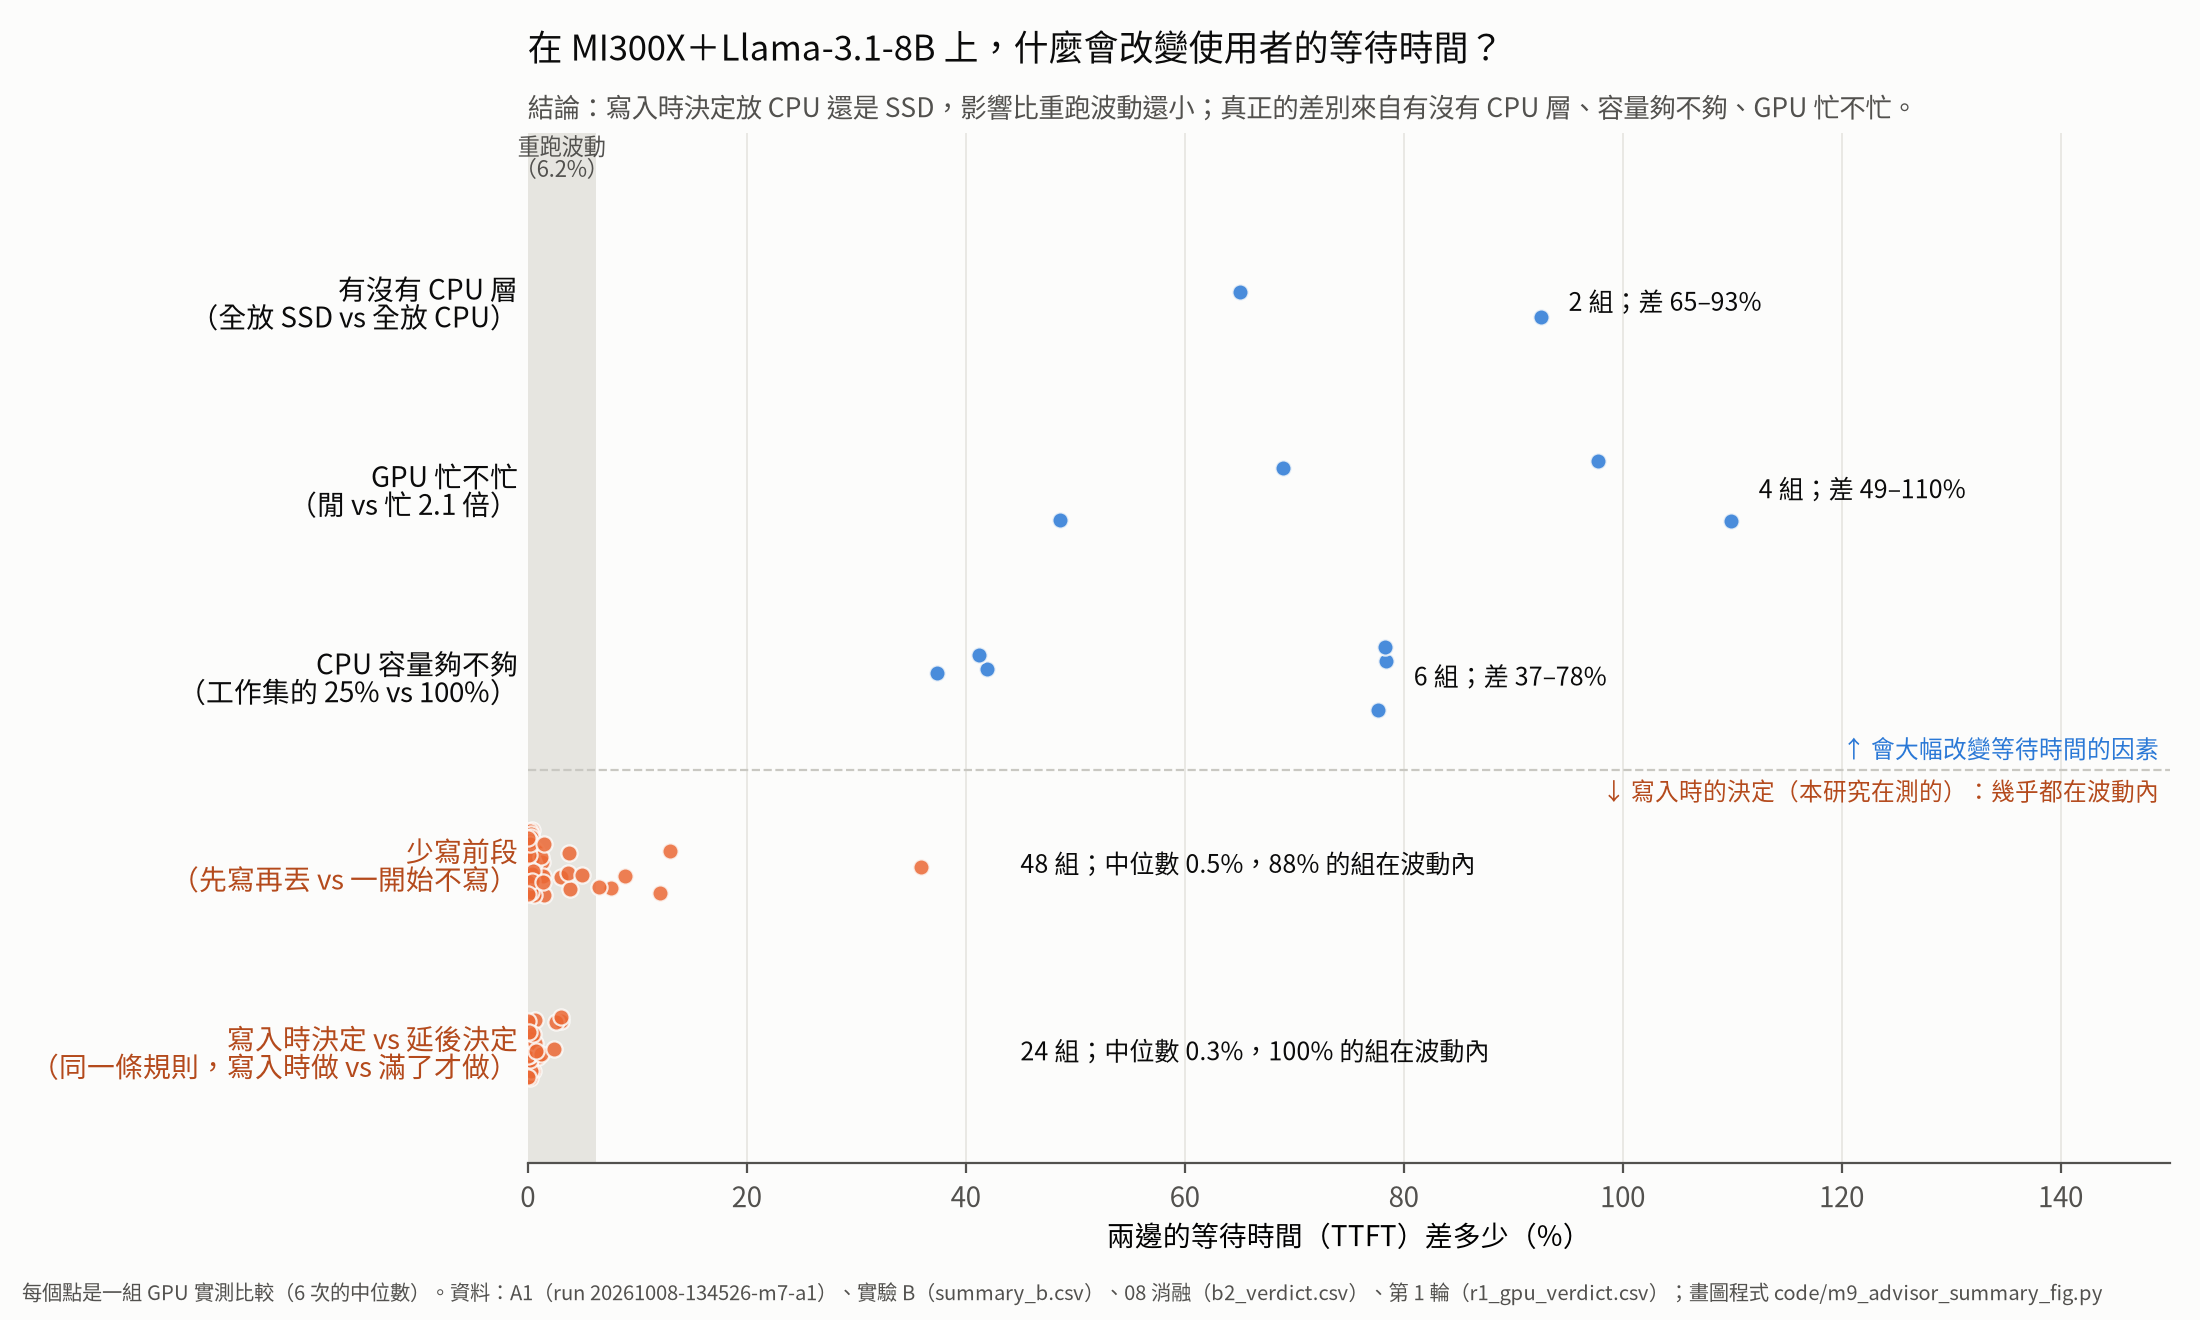
\includegraphics[width=\linewidth]{../report/figs/advisor_summary.png}
\caption{總覽：什麼會改變使用者的等待時間。每個點是一組 GPU 實測比較。寫入時的決定（橘色）幾乎都在重跑波動內；有沒有 CPU 層、容量夠不夠、GPU 忙不忙（藍色）才會大幅改變等待時間。}\label{fig:summary}
\end{figure}

%==========================================================
\sect{一、驗證的設定}

\begin{itemize}
\item \textbf{機器與模型}：AMD MI300X 單卡；Llama-3.1-8B，BF16；還原一律用 Cake。
\item \textbf{各層速度}：見表~\ref{tab:tier}。SSD 和 NFS 用限速器模擬，參數取實測最慢值 ×0.9。
\item \textbf{Context}：單一 session 為 4K--32K。多 session 實驗為 8 個 session，每個最多 4 輪，每輪加 8K（最長 32K）。
\item \textbf{重算 vs 載入}：見表~\ref{tab:restore}。以一段（512 token）來看，重算要 29--99 毫秒（越後面越貴），從 CPU 載入只要 1.8 毫秒。
\item \textbf{同一設定重跑的波動是 6.2\%}，之後的差距都要大過它才算數。
\end{itemize}

\begin{table}[h]
\centering
\begin{minipage}[t]{0.44\linewidth}
\centering
\caption{各層頻寬（GiB/s）}\label{tab:tier}
\begin{tabular}{lrr}
\toprule
層 & 讀 & 寫 \\
\midrule
GPU $\leftrightarrow$ CPU（PCIe 實測） & $\approx$50 & -- \\
CPU 層 & 35.4 & 35.5 \\
本地 SSD & 6.98 & 1.91 \\
NFS & 0.33 & 0.60 \\
\bottomrule
\end{tabular}
\end{minipage}\hfill
\begin{minipage}[t]{0.52\linewidth}
\centering
\caption{還原一個 32K session 要多久（秒；BF16，KV 約 4 GiB）}\label{tab:restore}
\begin{tabular}{lrrr}
\toprule
儲存層 & 只算 & 只載 & Cake \\
\midrule
本地 SSD 速度 & \multirow{2}{*}{3.76} & 0.66 & 0.57 \\
NFS 速度 & & 12.17 & 2.72 \\
\bottomrule
\end{tabular}

\vspace{2pt}
\note{註：本程式的重算比預設 vLLM 慢約 1.7--2 倍（第一階段拿來對照的 vLLM 剛好跑在它的慢路徑上）。把重算加快 2 倍再模擬一次，結論不變，但還沒有 GPU 確認。}
\end{minipage}
\end{table}

\subsect{Cake（最接近的 baseline）有跑通}
用 4K--32K × 7 種頻寬（0.33--11.6 GiB/s）共 28 組，檢查原論文的三個趨勢：
\begin{enumerate}
\item \textbf{context 越長，Cake 比「只算」快越多}：7 種頻寬全部成立。例如本地 SSD 速度下，從 3.1 倍增加到 6.7 倍。
\item \textbf{頻寬越快，Cake 比「只載」的好處越小}：最慢和最快兩端成立（NFS 速度 4.5--6.3 倍 → 100 Gbps 0.94--1.27 倍），中間的頻寬不完全照順序。
\item \textbf{Cake 不會比「只算」或「只載」慢}：28 組中 27 組成立。例外是 4K × 100 Gbps，Cake 慢 5.6\%：只有 8 段，兩條線同時跑的同步開銷大過好處。原論文的 GQA 模型（Llama-3.1-8B）在 32 Gbps 時也只有 0.98 倍。
\end{enumerate}

%==========================================================
\sect{二、實驗內容}

\subsect{（一）實驗設計}
會比較的做法如表~\ref{tab:strat}（都用 BF16，還原都用 Cake）。

\begin{table}[h]
\centering
\caption{比較的做法}\label{tab:strat}
\small
\begin{tabularx}{\linewidth}{l >{\raggedright\arraybackslash}X >{\raggedright\arraybackslash}X l}
\toprule
做法 & 寫入時 & CPU 滿了時 & 說明 \\
\midrule
全部都存（純 Cake） & 全部寫進 SSD & -- & Cake 原本的設定 \\
先寫再丟 & 先全部寫進 SSD，寫完再刪掉前段（最後留下的和「一開始不寫」一樣，只差前段有沒有先寫過一次） & -- & 老師點名；看「少寫」本身有沒有用 \\
一開始不寫 & 前段不寫，其他寫進 SSD & -- & 老師點名；我原本的設計 \\
寫穿 & CPU 和 SSD 各寫一份 & 刪掉最久沒用的 CPU 那份 & 業界預設（vLLM、LMCache） \\
延後寫入 & 只寫進 CPU & 這時才把最久沒用的搬到 SSD & 老師點名 \\
延後寫入＋成本感知 & 只寫進 CPU & 這時才把最好重算的（前段）搬到 SSD & 兩個簡單方法的組合 \\
\textbf{依位置放（我的方法）} & 後段寫進 CPU，前段寫進 SSD & 同上 & 本研究 \\
\bottomrule
\end{tabularx}
\end{table}

四組實驗：
\begin{itemize}
\item \textbf{實驗 A}（單一 session，回答 Q1、Q2）：長度 4K--32K；GPU 分閒、忙 1.5 倍、忙 2.1 倍（同一張卡上跑背景負載，讓重算變慢）；SSD 層分本地 SSD、NFS；使用者分「寫完才回來」和「寫入中就回來」；每格 6 次，共 1,440 次還原。
\item \textbf{實驗 B}（多 session、CPU 容量有限，回答「簡單策略會不會追平」）：8 個 session 輪流回來，每個最多 4 輪、每輪加 8K；CPU 容量設成工作集的 25\%、50\%、100\%。
\item \textbf{08 消融}：把對我的方法最有利的條件疊在一起再測：CPU 慢（3.69 GiB/s，vLLM 實測）、容量緊、搬移會卡住請求、一次寫一大段文件。先用模擬篩，再上 GPU。
\item \textbf{第 1 輪}：模擬篩出唯一有機會的設定，上 GPU 跑 5 個 seed。
\end{itemize}

\subsect{（二）結果}

\textbf{1. 省下的寫入有沒有縮短等待？——幾乎沒有（表~\ref{tab:q1}）}

「先寫再丟」和「一開始不寫」最後留下的東西一樣，只差前段有沒有先寫過一次。32K 時，「一開始不寫」在 NFS 上少寫了 64 段裡的 51 段（約 80\%），在本地 SSD 上少寫 13 段。

\begin{table}[h]
\centering
\caption{回來請求的等待時間 TTFT（毫秒；GPU 閒；6 次的中位數）}\label{tab:q1}
\begin{tabular}{llrrrr}
\toprule
\multirow{2}{*}{SSD 層} & \multirow{2}{*}{context} & \multicolumn{2}{c}{寫完才回來} & \multicolumn{2}{c}{寫入中就回來} \\
\cmidrule(lr){3-4}\cmidrule(lr){5-6}
 & & 先寫再丟 & 一開始不寫 & 先寫再丟 & 一開始不寫 \\
\midrule
\multirow{4}{*}{本地 SSD} & 4K & 103 & 95 & 172 & \textbf{149（−13\%）} \\
 & 8K & 156 & 156 & 302 & 291 \\
 & 16K & 292 & 288 & 577 & 582 \\
 & 32K & 533 & 580 & 1,192 & 1,195 \\
\midrule
\multirow{4}{*}{NFS} & 4K & 250 & 340 & 345 & 345 \\
 & 8K & 525 & 533 & 672 & \textbf{591（−12\%）} \\
 & 16K & 1,206 & 1,189 & 1,313 & 1,248 \\
 & 32K & 2,746 & 2,745 & 3,114 & \textbf{2,910（−6.5\%）} \\
\bottomrule
\end{tabular}

\vspace{2pt}
\note{粗體：差距大於重跑波動 6.2\%，而且 6 次重跑的範圍不重疊；其他格的差距都在波動內。GPU 忙的 32 組見附錄表~A1。}
\end{table}

\begin{itemize}
\item \textbf{寫完才回來}：兩種做法幾乎一樣。例如 NFS、32K，少寫了 80\% 的資料，等待時間還是 2,746 vs 2,745 毫秒。
\item \textbf{寫入中就回來}：使用者在上一輪的資料還沒寫完時就回來，硬碟要同時寫和讀，所以讀變慢（例：本地 SSD、32K，從 533 毫秒變成 1,192 毫秒）。這時「一開始不寫」雖然寫得比較少，但大多數情況下，回來時寫入一樣還沒結束，硬碟一樣被佔著，所以只有 3 組明顯變快（6.5--13\%）。
\item \textbf{GPU 忙的時候}（另外 32 組）：兩種做法的差距都在 ±3.8\% 以內，沒有一組明顯變快。
\item \textbf{結論}：少寫本身不會讓等待變短，只有少寫到讓寫入在使用者回來前就寫完，才有一點幫助。
\end{itemize}

\textbf{2. GPU 閒的時候，不存前段沒差；GPU 忙的時候，代價很大（表~\ref{tab:q2}、圖~\ref{fig:breakdown}）}

\begin{table}[h]
\centering
\caption{「一開始不寫」比「全部都存」慢多少（正值＝較慢）}\label{tab:q2}
\begin{tabular}{llrrr}
\toprule
SSD 層 & context & GPU 閒 & GPU 忙 1.5 倍 & GPU 忙 2.1 倍 \\
\midrule
\multirow{2}{*}{本地 SSD} & 16K & −1.1\%（不顯著） & +36.2\% & +52.0\% \\
 & 32K & +7.1\%（不顯著） & +29.2\% & +66.4\% \\
\midrule
\multirow{2}{*}{NFS} & 16K & −0.8\%（不顯著） & +13.2\% & +24.9\% \\
 & 32K & +0.9\%（不顯著） & +14.2\% & +30.5\% \\
\bottomrule
\end{tabular}
\end{table}

\begin{itemize}
\item \textbf{GPU 閒}：Cake 本來就會重算前段，所以前段存不存都一樣。
\item \textbf{GPU 忙}：「全部都存」可以讓 Cake 少算幾段、改從 SSD 搬（本地 SSD、32K 時，從重算 13 段降到 7 段）。「一開始不寫」沒有備份，只能硬算 13 段，所以 16K 以上慢 13--66\%。
\item 所以我把設計改成「每段都存，只改放的位置」。
\item 圖~\ref{fig:breakdown} 把每次還原拆成「GPU 重算」和「I/O 載入」兩條線，可以直接看到省下的 I/O 和增加的計算。
\end{itemize}

\textbf{3. 和延後寫入、成本感知逐出比較：簡單策略追平（表~\ref{tab:q3}）}

實驗 B（8 個 session）：
\begin{itemize}
\item 依位置放 vs 延後寫入＋成本感知：所有設定只差 −3.0\%～+0.3\%。
\item CPU 容量 25\% 時，依位置放反而比最好的簡單策略慢 29\%；50\% 時慢 3.7\%；100\% 時差 0.4\%。
\end{itemize}

\begin{table}[h]
\centering
\caption{「寫入時決定」vs 簡單策略、延後版（GPU 實測，共 36 組比較）}\label{tab:q3}
\small
\begin{tabular}{lcccc}
\toprule
實驗 & 比較組數 & 贏簡單策略 $\geq$5\% & 贏延後版 $\geq$5\% & 兩邊都贏 $\geq$5\% \\
\midrule
實驗 B（CPU 容量 25／50／100\%） & 15 & 0 & 0 & 0 \\
08 消融（有利條件疊在一起） & 16 & 1 & 5 & 0 \\
第 1 輪（5 個 seed） & 5 & 0 & 0 & 0 \\
\midrule
合計 & 36 & 1 & 5 & \textbf{0} \\
\bottomrule
\end{tabular}

\vspace{2pt}
\note{簡單策略：寫穿、延後寫入、成本感知逐出等，取最好的。延後版：同一條規則（前段放 SSD、後段放 CPU），但等 CPU 滿了才做。}
\end{table}

\begin{itemize}
\item 唯一贏簡單策略的那一組（快 18.9\%），只比延後版快 0.7\%，換一個 seed 就不見了：贏的是規則本身，不是「寫入時」。
\item 贏延後版的 5 組，都沒贏簡單策略（−4.8\%～+0.4\%）。它們都在「搬移會卡住請求」的設定，那裡寫穿本來就最快。
\item 之後又從多個角度（多人同時使用、真實 vLLM、真實 trace、換模型等）和新的 seed 重測，結論都一樣。
\end{itemize}

\subsect{（三）小結}
\begin{itemize}
\item \textbf{為什麼延後版一樣好}：決定哪幾段放 SSD，看的是「這段在第幾頁」。這個資訊不會變，等 CPU 滿了要搬的時候一樣知道。所以「CPU 滿了才把前段搬去 SSD」，最後的擺法和「一寫進來就把前段放 SSD」一模一樣，速度也一樣。
\item \textbf{真正影響等待時間的}：資料在不在 CPU（CPU 比 SSD 快很多）、CPU 放不放得下、GPU 忙不忙（圖~\ref{fig:summary}）。寫入的時機幾乎沒有影響。
\item \textbf{寫入時唯一要注意的}：不要一開始就不存。沒存的段之後就沒了，GPU 忙的時候只能重算，會慢 13--66\%（表~\ref{tab:q2}）。所以寫入時每一段都存，等 CPU 滿了再搬到 SSD 就好。
\end{itemize}

%==========================================================
\sect{附圖}
\begin{figure}[h]
\centering
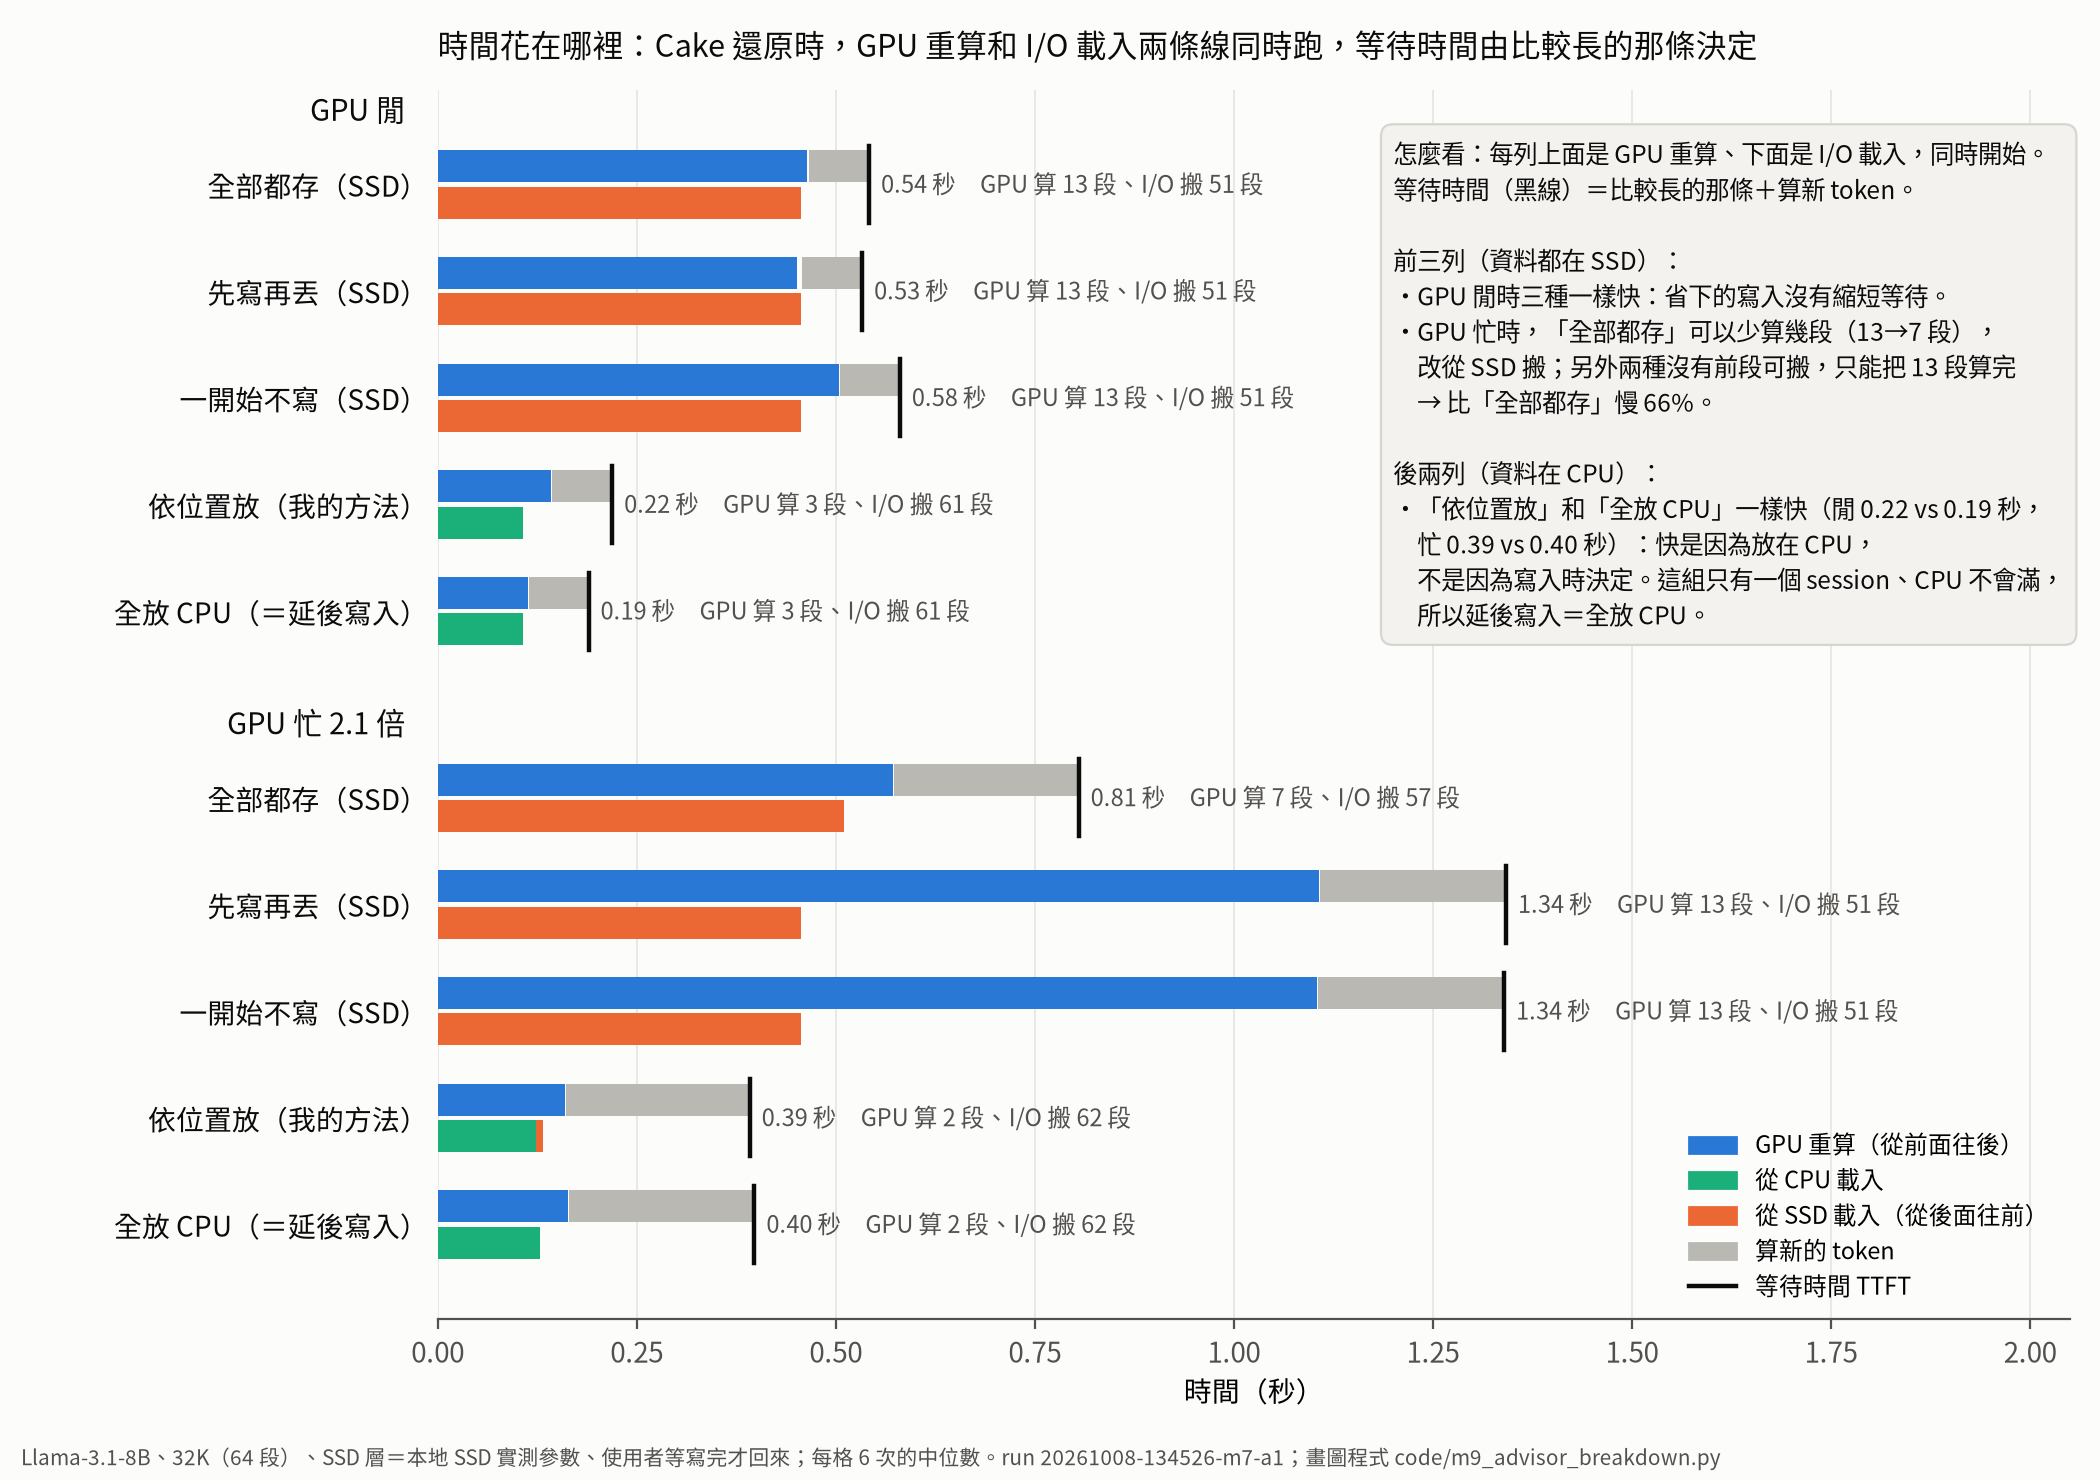
\includegraphics[width=\linewidth]{../report/figs/advisor_breakdown.png}
\caption{時間花在哪裡（32K、本地 SSD、使用者等寫完才回來）。每列上面是 GPU 重算、下面是 I/O 載入，兩條同時跑，等待時間由比較長的那條決定。前三列資料在 SSD：GPU 閒時一樣快，GPU 忙時沒存前段的只能把 13 段算完。後兩列資料在 CPU：「依位置放」和「全放 CPU（＝延後寫入）」一樣快。}\label{fig:breakdown}
\end{figure}

\begin{figure}[h]
\centering
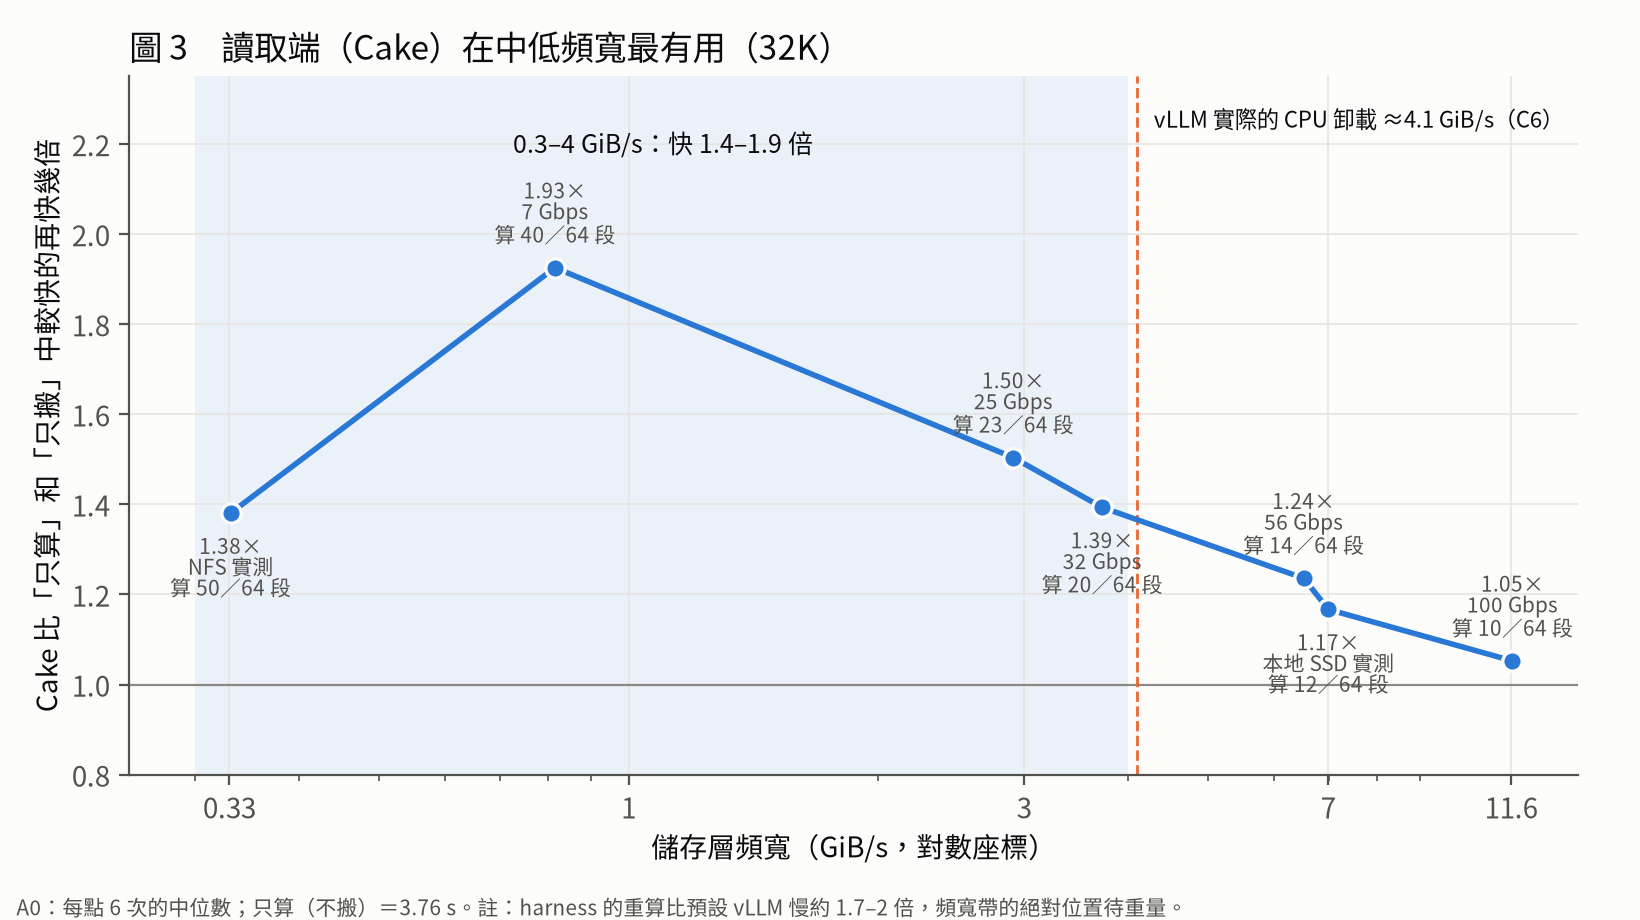
\includegraphics[width=0.82\linewidth]{../report/figs/advisor_fig3.png}
\caption{讀取端（Cake）在中低頻寬（0.3--4 GiB/s）最有用：比「只算」或「只載」中較快的再快 1.4--1.9 倍；11.6 GiB/s 時只快 5\%。vLLM 實際的 CPU 卸載約 4.1 GiB/s，正好落在這個範圍。}\label{fig:cake}
\end{figure}

%==========================================================
\clearpage
\sect{附錄：完整數字}

\begin{center}
\renewcommand{\thetable}{A1}
\captionof{table}{先寫再丟 vs 一開始不寫，GPU 忙時的等待時間 TTFT（毫秒；6 次的中位數）}\label{tab:a1}
\small
\begin{tabular}{lllrrrr}
\toprule
\multirow{2}{*}{GPU} & \multirow{2}{*}{SSD 層} & \multirow{2}{*}{context} & \multicolumn{2}{c}{寫完才回來} & \multicolumn{2}{c}{寫入中就回來} \\
\cmidrule(lr){4-5}\cmidrule(lr){6-7}
 & & & 先寫再丟 & 一開始不寫 & 先寫再丟 & 一開始不寫 \\
\midrule
\multirow{8}{*}{忙 1.5 倍} & \multirow{4}{*}{本地 SSD} & 4K & 145 & 146 & 198 & 198 \\
 & & 8K & 203 & 203 & 357 & 352 \\
 & & 16K & 432 & 445 & 717 & 720 \\
 & & 32K & 821 & 828 & 1,399 & 1,404 \\
\cmidrule(lr){2-7}
 & \multirow{4}{*}{NFS} & 4K & 414 & 412 & 398 & 400 \\
 & & 8K & 837 & 826 & 825 & 823 \\
 & & 16K & 1,777 & 1,798 & 1,782 & 1,787 \\
 & & 32K & 4,100 & 4,083 & 4,234 & 4,078 \\
\midrule
\multirow{8}{*}{忙 2.1 倍} & \multirow{4}{*}{本地 SSD} & 4K & 251 & 252 & 272 & 271 \\
 & & 8K & 358 & 354 & 515 & 496 \\
 & & 16K & 742 & 739 & 912 & 916 \\
 & & 32K & 1,342 & 1,339 & 1,654 & 1,652 \\
\cmidrule(lr){2-7}
 & \multirow{4}{*}{NFS} & 4K & 664 & 662 & 655 & 658 \\
 & & 8K & 1,318 & 1,315 & 1,318 & 1,322 \\
 & & 16K & 2,814 & 2,807 & 2,800 & 2,802 \\
 & & 32K & 5,975 & 5,996 & 5,992 & 5,987 \\
\bottomrule
\end{tabular}

\vspace{2pt}
\note{32 組的差距都在 ±3.8\% 以內，沒有一組明顯變快。}
\end{center}

\vspace{10pt}
{\footnotesize
\setlength{\tabcolsep}{2.5pt}
\renewcommand{\thetable}{A2}
\begin{longtable}{r l >{\raggedright\arraybackslash}p{5.7cm} l l r r r r r}
\caption{表~\ref{tab:q3} 的 36 組比較（回來請求 TTFT 中位數，秒）}\label{tab:a2}\\
\toprule
\# & 實驗 & 設定 & 寫入時 & 最好的簡單 & \multicolumn{3}{c}{TTFT（秒）} & \multicolumn{2}{c}{寫入時決定快多少} \\
\cmidrule(lr){6-8}\cmidrule(lr){9-10}
 & & & 策略 & 策略 & 寫入時 & 簡單 & 延後版 & vs 簡單 & vs 延後版 \\
\midrule
\endfirsthead
\toprule
\# & 實驗 & 設定 & 寫入時 & 最好的簡單 & 寫入時 & 簡單 & 延後版 & vs 簡單 & vs 延後版 \\
\midrule
\endhead
\csname @@input\endcsname table36_rows.tex 
\bottomrule
\end{longtable}
}
\vspace{-6pt}
\note{設定欄依序是：負載型態、CPU 層頻寬（GiB/s，沒寫的是 35.4）、SSD 層（本地 SSD 或 NFS）、CPU 容量（佔工作集的比例）、workload seed。08 的 16 組都是「搬移會卡住請求」的設定；「SSD 50\%」＝SSD 容量也有限。\\
正值＝寫入時決定比較快；粗體＝快 $\geq$5\%。「兩邊都快 $\geq$5\%」的組數是 0。\\
實驗 B 是 8 個 session 的對話型負載（第一階段）；08 消融刻意疊加對寫入時決定有利的條件；第 1 輪是模擬篩出的唯一設定。\\
寫入時策略：S5＝依位置放（後段放 CPU、前段放 SSD，CPU 滿了照成本感知搬）；S5L＝同樣依位置放，但 CPU 滿了先搬最久沒用的 session；S5c＝全部放 CPU，另外在寫入時把前段先複製一份到 SSD。\\
延後版：實驗 B 為 S4+（只寫 CPU，滿了才把前段搬到 SSD）；08 與第 1 輪為 S4B（只寫 CPU，滿了才照同一條位置規則搬）。\\
簡單策略：S1＝寫穿＋LRU；S2b＝寫穿＋成本感知逐出；S4＝延後寫入＋LRU；S4+＝延後寫入＋成本感知；S4+P＝延後寫入＋Pensieve 式（成本×閒置時間）；S4L＝延後寫入，搬最久沒用的 session、從前段開始。}

\vspace{6pt}
{\raggedright\sloppy\note{資料來源：表~\ref{tab:q1}、A1：\texttt{results/m7\_write\_policy\_mi300x/summary\_a1\_pairs.csv}（run 20261008-134526-m7-a1）；表~\ref{tab:restore}：\texttt{a0.csv}（run 20261008-133544-m7-a0）；表~\ref{tab:q2}：07 報告 §5；表~\ref{tab:q3}、A2：\texttt{summary\_b.csv}、\texttt{b2\_verdict.csv}、\texttt{b2\_summary.csv}、\texttt{r1\_gpu\_verdict.csv}（整理：\texttt{code/m9\_advisor\_table36.py}）；圖：\texttt{code/m9\_advisor\_summary\_fig.py}（run 20261013-030010-advisor-summary）、\texttt{m9\_advisor\_breakdown.py}（run 20261013-025740-advisor-breakdown）、\texttt{m9\_advisor\_figs.py}（run 20261012-152226-advisor-figs）。}\par}

\end{document}
